\documentclass[a4paper,11pt,fleqn, titlepage]{article}

\usepackage[utf8]{inputenc}
\usepackage[swedish]{babel}
\usepackage[lighttt]{lmodern}
\usepackage{parskip}
\usepackage{amsmath}
\usepackage{amssymb}
\usepackage{amsthm}
\usepackage{listings}
\usepackage{graphicx}

\author{Andreas Hagesjö \and Daniel Pettersson \and
Magnus Hagmar \and Niclas Ogeryd \and Robert Nyquist}

\title{Modell över Sveriges primärenergitillförsel \\ Kurs ENM155} 


\begin{document}
\maketitle

\section{Introduktion}
Denna rapport innehåller en enkel modell utav Sveriges energisystem som det
ser ut idag. Modellen visar hur olika primäreneriger födelas på de tre
sektorerna industri, transport och bostäder samt en uppskattning utav
Sveriges totala primärenergitillförsel.


\section{Metod}
Modellen är nerbruten i tre delar, industri, transport och bostäder som är
de olika sektorerna. För varje sektor så listas alla primärenergier som
birdrar till respektive sektor. Varje primärenergi går sedan vidare till de
olika sekundärenergierna som den bidrar till. Varje sekundärenergi går
vidare till sektorn, alternativ till en ny sekundärenergi som i sin tur går
vidare till en sektor eller ytterligare en sekundärenergi.

\begin{itemize}
\item Då vi har brutit ner modellen i sektorer så följer de inte diagrammet
	i Figur 1 i lab PM. Istället så ger flödesschemat i Appendix
	\ref{app:schema} en direkt bild utav strukturen på våran
	implementation.


\item Modellen är byggd så att det går att ta reda på tillförseln av varje
	enskild primärenergi samt vilka typer av primärenergi, och mängedn,
	varje enskild sektor använder. Det går även att räkna ut värden på
	sekundärenergierna för varje sektor med hjälp av modellen.

\item Då varje sektor innehåller alla primärenergier och sekundärenergier
	som bidrar så blir det väldigt enkelt att addera nya energier. Den nya
	energin läggs till i sektorn den bidrar till och går sedan vidare till
	en sekundärenerig eller sektorn.
\end{itemize}

\subsection{Matematisk modell}
Vi definerar ett utryck för att beräkna elen i transport samt
industrisektorn, som vi sedan referenserar för att minska längden på det
totala uttrycket.

I våra ekvationer betyder $E_{fe}$ energin från fossila bränslen omvandlat
till el. Samma sätt med $E_{fjv}$, fjärrvärme till värme, $E_{ffj}$, fossil
till fjärvärme etc.

\newpage

\subsection{Bostäder}
\begin{align*}
	EL &= \frac{\frac{E_v k_{ev}}{\varphi_{ev}} + \frac{E_v k_{fjv}
	k_{vp}}{\varphi_{fjv} \varphi_{vp} \varphi_{trans}} +
	E_e}{\varphi_e \varphi_{trans}} \\
\intertext{Fossila bränslen}
	E_f &= \frac{E_v k_{fv}}{\varphi_{fv}} + \frac{E_v k_{fjv}
	k_{ffj}}{\varphi_{fjv} \varphi_{ffj} \varphi_{trans}} + EL
	\cdot \frac{k_{fe}}{\varphi_{fe}} \\
\intertext{Biobränslen}
	E_b &= \frac{E_v k_{bv}}{\varphi_{bv}} + \frac{E_v k_{fjv}
	k_{bfj}}{\varphi_{fjv} \varphi_{bfj} \varphi_{trans}} + EL
	\cdot \frac{k_{be}}{\varphi_{be}} \\
\intertext{Vindkraft}
	E_{vind} &= EL \cdot \frac{k_{vind}}{\varphi_{vind}} \\
\intertext{Vattenkraft}
	E_{vatten} &= EL \cdot \frac{k_{vatten}}{\varphi_{vatten}} \\
\intertext{Kärnkraft}
	E_{karn} &= EL \cdot \frac{k_{karn}}{\varphi_{karn}} \\
\intertext{Spillvärme (inte en riktig energi, men måste tas med i beräkningarna)}
	E_{spill} &= EL \cdot \frac{k_{spill}}{\varphi_{spill}} \\
\end{align*}


\subsection{Transport}
\begin{align*}
	E_f &= \frac{E_t k_f}{\varphi_f \varphi_{drivmedel}} \\
	E_b &= \frac{E_t k_b}{\varphi_b \varphi_{drivmedel}} \\
\end{align*}


\subsection{Industri}
Industrisektorn skiljer sig från bostadssektorn genom att det inte finns
någon eluppvärmning, annars är de två sektorerna lika.
\begin{align*}
	EL &= \frac{\frac{E_v k_{ev}}{\varphi_{ev}} + E_e}{\varphi_e
	\varphi_{trans}} \\
\end{align*}


\section{Resultat}

I tabell \ref{resultat} visas den totala energitillförseln samt varje
enskild energikällas tillförsel.
\begin{table}[h!]
	\centering
	\begin{tabular}{| l | r |}
		\hline
		Energikälla      & Tillförsel \\ \hline
		Fossila bränslen & 201.483 TWh \\
		Biobränsle       & 147.288 TWh \\
		Vindkraft        &   4.187 TWh \\
		Vattenkraft      &  71.491 TWh \\
		Kärnkraft        & 174.638 TWh \\ \hline
		Totalt           & 649.561 TWh \\ \hline
	\end{tabular}
	\caption{Resultat}
	\label{resultat}
\end{table}


\newpage
\appendix

\section{Flödesschema}
\begin{figure}[h!]
	\centering 
	\vspace*{0cm}
	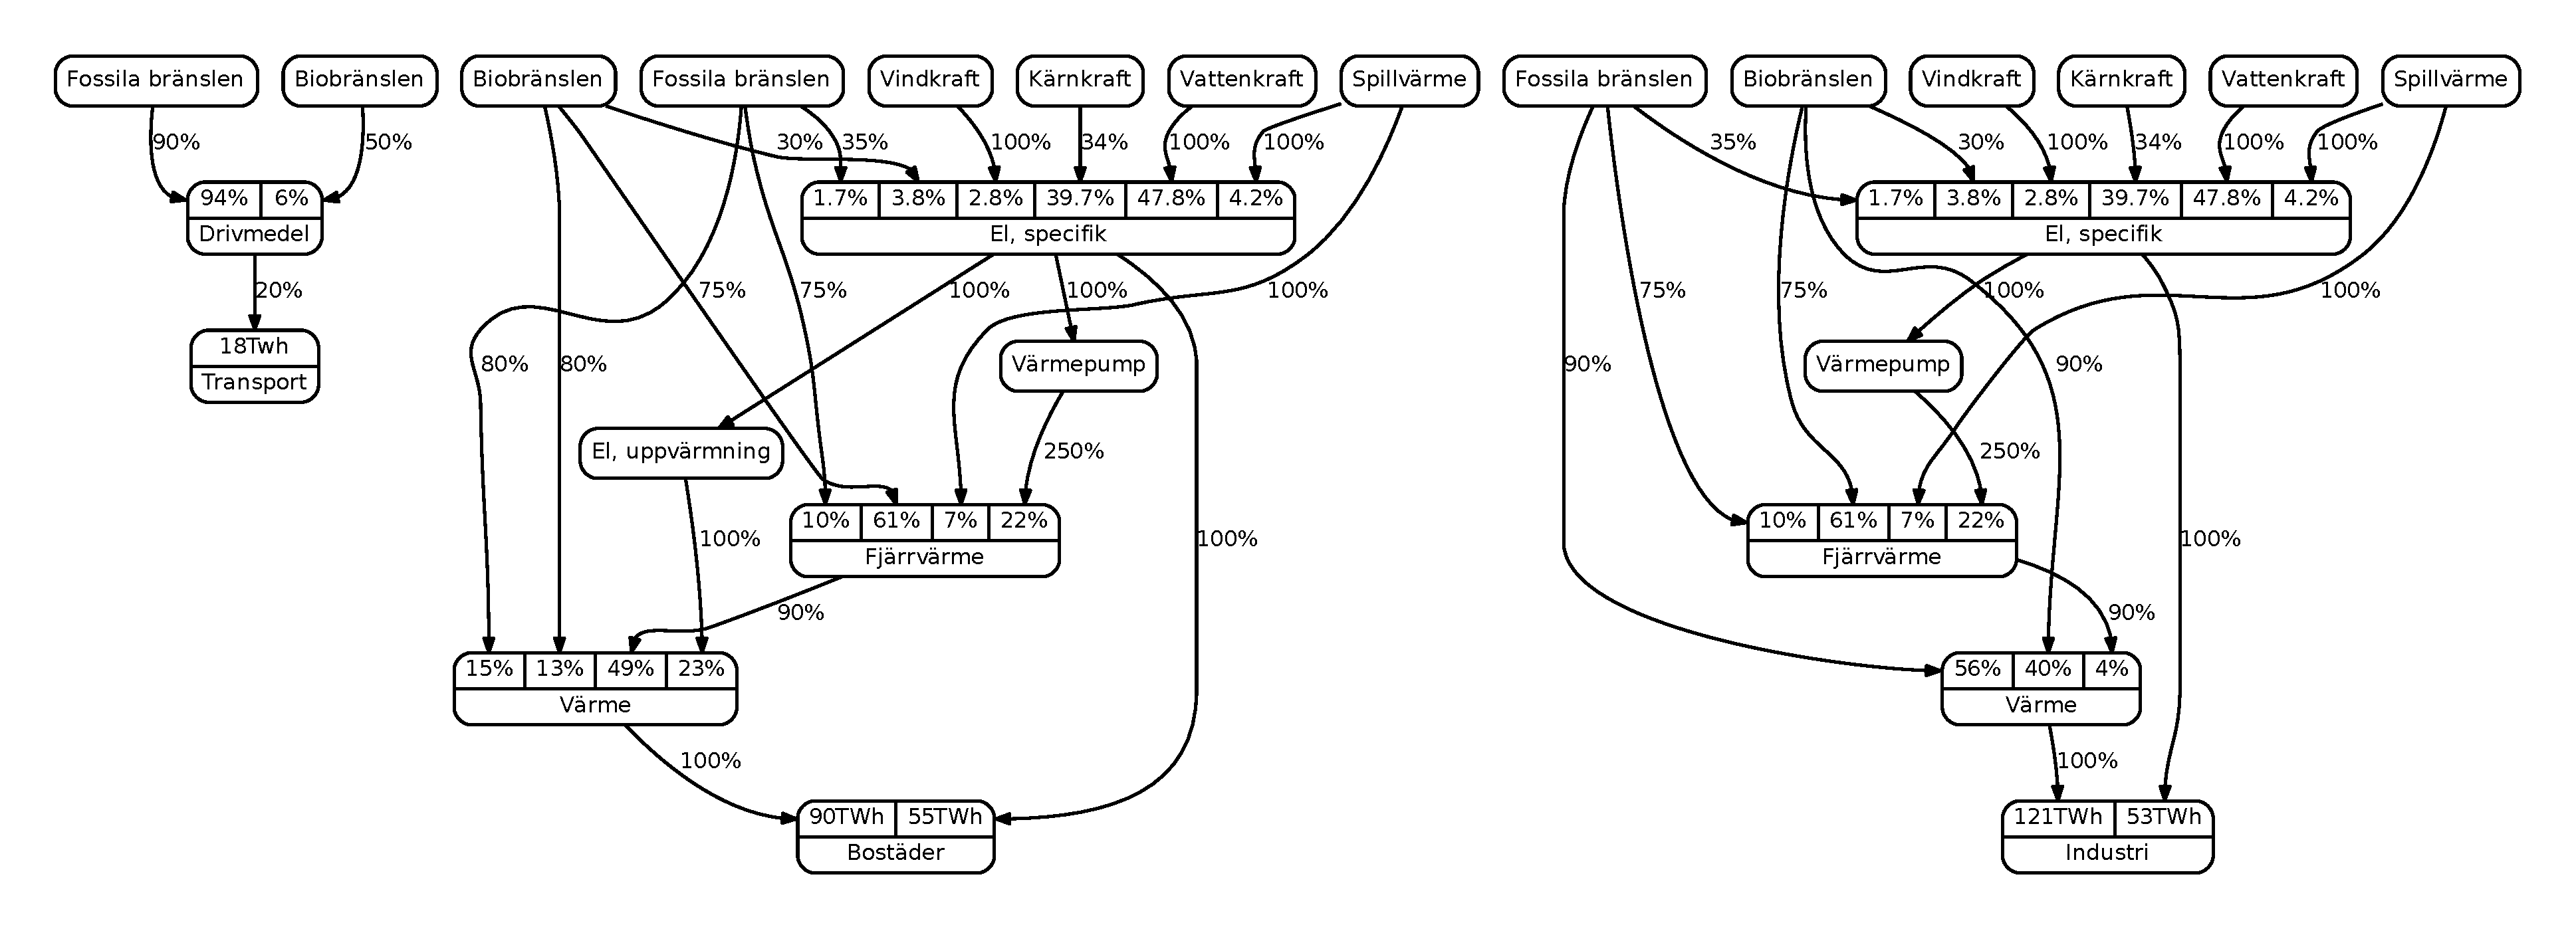
\includegraphics[width=0.6\paperheight,angle=270]{diagram.pdf}
	\label{app:schema}
	\caption{Flödesschema över energianvändning i Sverige.}
\end{figure}

\newpage

\section{Programkod}
Bifoga koden

\end{document}

